The code is divided into three parts\-: the (optional) parameters file, user defined functions, and core functions. The parameters file includes the definition of parameters used in the simulation (mesh refinement, time step size, material parameters, etc.). The user defined functions is a list of functions that can/must be defined by the user. The {\ttfamily define\-Parameters} and {\ttfamily residual} functions (italicized) require a user definition; the remaining functions have default definitions that can be overridden by the user if desired. These user functions are called by the core functions, as shown in the following diagram.

\begin{center}

\begin{DoxyImageNoCaption}
  \mbox{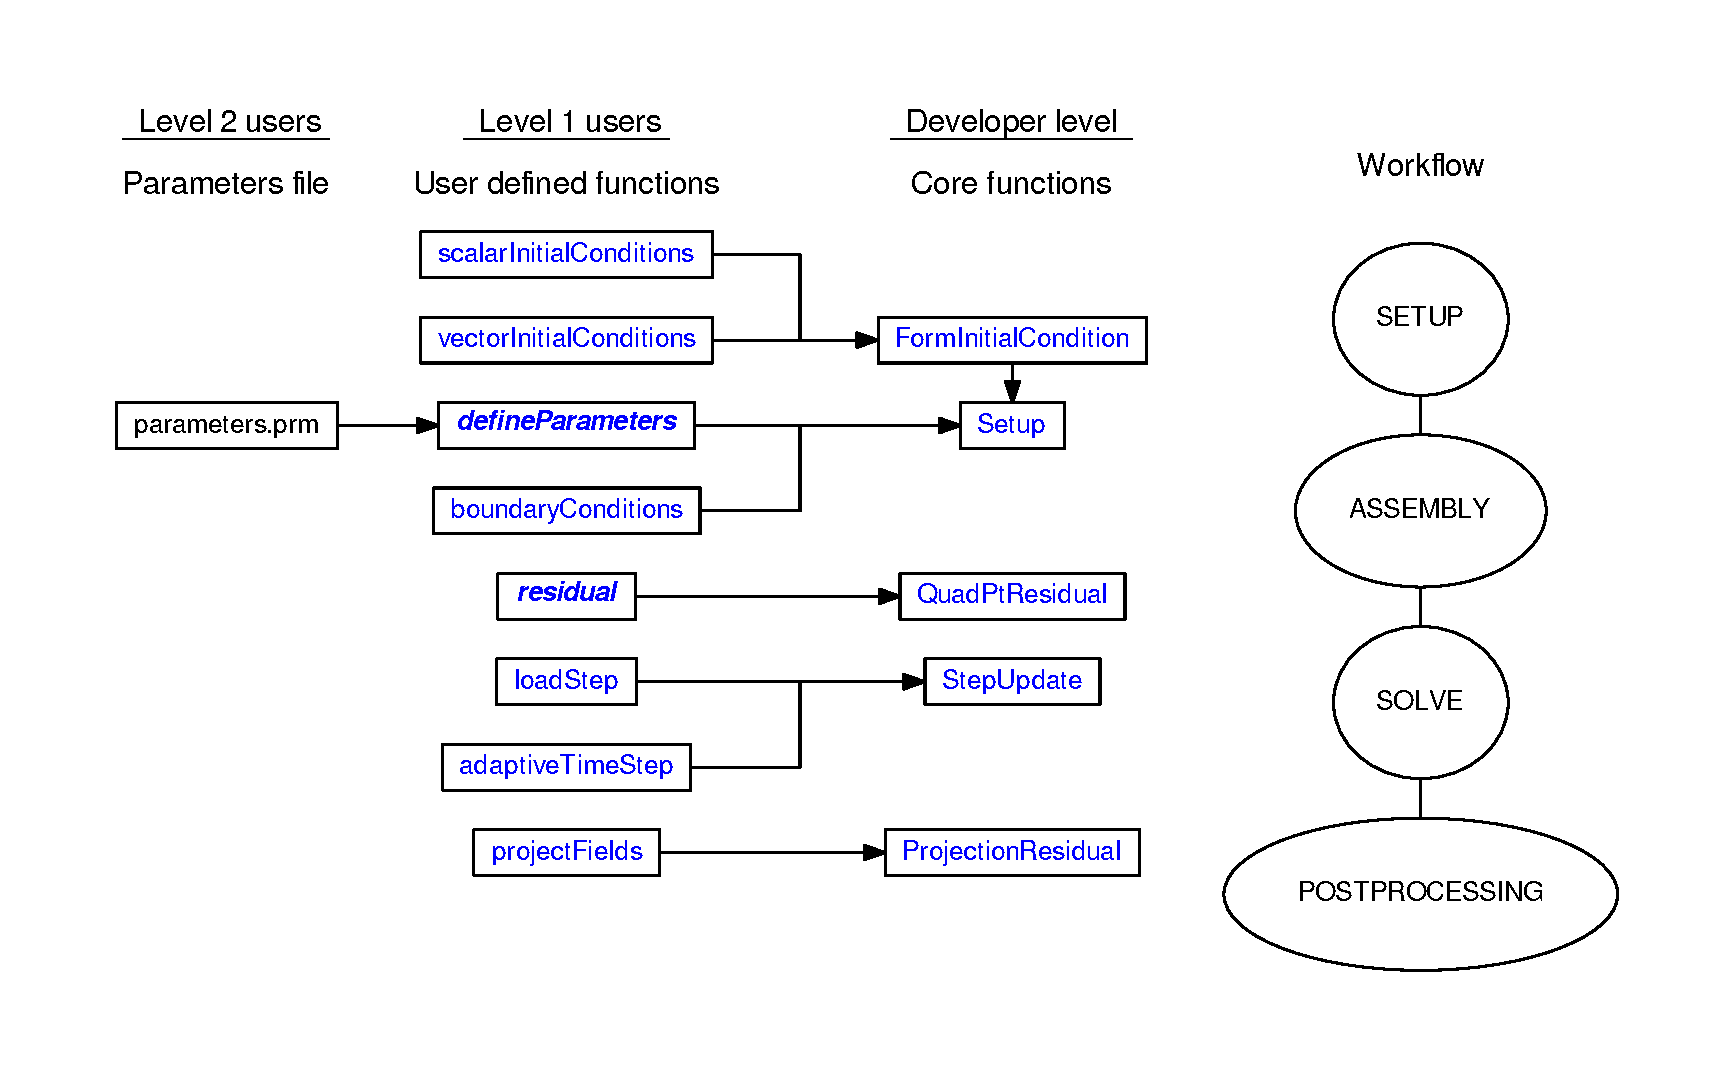
\includegraphics[width=\textwidth,height=\textheight/2,keepaspectratio=true]{dot_inline_dotgraph_1}}
\end{DoxyImageNoCaption}
\end{center}
 